\documentclass{article}
\usepackage[utf8]{inputenc}
\title{Vidio 3: How Not To Estimate Risk}
\author{wbg231 }
\date{December 2022}
\newcommand{\R}{$\mathbb{R}$}
\newcommand{\B}{$\beta$}
\newcommand{\A}{$\alpha$}
\newcommand{\D}{\Delta}

\newcommand{\avector}[2]{(#1_2,\ldots,#1_{#2})}
\newcommand{\makedef}[2]{$\textbf{#1}$:#2 }
\usepackage{tikz,graphicx,hyperref,amsmath,amsfonts,amscd,amssymb,bm,cite,epsfig,epsf,url}

\begin{document}

\maketitle

\section{introduction}
\begin{itemize}
\item \href{https://www.youtube.com/watch?v=p_QTXkKod4k&list=PLBEf5mJtE6KuZ5NBQMuWIMsiOOrV9ibzm&index=72}{video link}
\item the central limit theorem tells us that the sum of independent quantities are approximately Gaussian, but this only holds if the quantities are actually indented if this assumption is violated things fail 
\ection{central limit theorem}
\item so the central limit theorem stats if we have \textbf{independent} random variables $\Tilde{x}_1...$ with mean $\mu$ and standard deviation $\sigma$
\item the sample mean $\Tilde{m}_{n}=\frac{1}{n}\Sigma_{i=1}^{n}x_i$
\item will be unbiased $E[Tilde{m}_{n}]=\mu$
\item and will have standard error equal to $se(Tilde{m}_{n})=\frac{\sigma}{\sqrt{n}}$
\item as n approaches infinity our sample mean will converge in distribution to a Gaussian with mean $\mu$ and standard deviation $\frac{\sigma}{\sqrt{n}}$
\section{mortgage example}
\subsection{set up}
\item we have n subprime (bad) mortgages 
\item the probability that each bower defaults is $\frac{2}{3}$
\item we want to build a low risk investment out of this 
\subsection{cauterized mortgage obligation}
\item idea we dive the mortgages into ten tranches that suffer loss sequentially
\item so if less 10 percent of the mortgages fail then only trench 1 is affected 
\item if less than 90 percent of mortgages fail then trench 10 is not effected. this called the senior tranche. this is a secure investment 
\item lets think about the risk of the senior tranche
\section{borrowers default independently}
\subsection{borrowers default independently}
\item supposes that borrowers default independently for now 
\item in that case the number of defaults $\Tilde{d}$ among n mortgages is a binomial with parameters n and $\tehat=2/3$
\item then the likelihood that the Senior tranche losses money is $P(\Tilde{d}>.9n)$ we can approx this with a standardized Gaussian 
\item and use that to write $P(\Tilde{d}>.9n)=P(\frac{\Tilde{d}-\theta n}{\sqrt{(\theta)(1-\theta)(n)}}>\frac{.9(n)-\theta n}{\sqrt{(\theta)(1-\theta)(n)}})\approx P(\Tilde{z}>,49\sqrt{n})$ where we have standardized both sides and z is a standard Gaussian  
\item for n=100 this probability is around $10^{-7}$
\item so the number of defaults will be distributed like this \\ 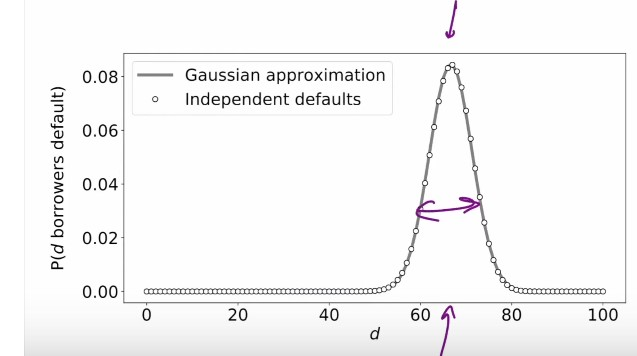
\includegraphics[width=10cm]{notes/week_4/vidio 3:How Not To Estimate Ris/immages/v_3_1.jpg}
\item and we are looking the likelihood of being grater than 90 of the lenders defaulting is essentially zero
\item this was how a lot of mortgages and loans were done prior to the 2008 financial crisis
\subsection{what could go wrong}
\item the problem is mortgages are not independent 
\item there was a finical crisis and all the mortgages failed at once. 
\item in real life the models did not assume mortgage Independence, this is just a cartoon example
\section{borrowers don't default indecently}
\subsection{borrowers don't default indecently}
\item suppose that the chance of default depends on the economic context.
\item say that there is a random variable $\Tilde{r}$ that represents where there is a recession. so $\Tilde{r}=0$ means economy is strong $\Tilde{r}=1$ means economic disaster
\item and further assume that the pdf of r is $f_{\Tilde{r}}(r)=2r$ for $r\om[0,1]$ (r is continuous)

\item conditioned on $\Tilde{r}=r$ each borrower defaults with probability r
\item so each default given the state of the economy is r  is a Bernoulli with parameter r 
\item $P(borrower defualt)=P(\Tilde{b}=1)=\int_{r=-\infty}^{\infty}P_{b|r}(1|r)f_{r}(r)dr=\int_{r=-\infty}^{\infty}r2rdr=\int_{0}^{1}2r^2dr=\frac{2}{3}$
\item so we have the same probability of default for each individual lender as we had in the case of Independence 
\item lets assume that defaults are conditionally independent given economic context
\item conditioned on $\Tilde{r}=r$ the number of defaults is binomial with parameters n and r 
\item $P_{\Tilde{d}}(d)=\int_{r=-\infty}^{\infty}f(r=r,d=d)dr=\int_{r=-\infty}^{\infty}f(d=d|r)f_{r}(r)dr=2r\begin{pmatrix}n\\d\end{pmatrix} r^{d}(1-r)^{n-d}dr$ this is a messy integral that ends up as $\frac{2(d+1)}{(n+1)(n+2)}$
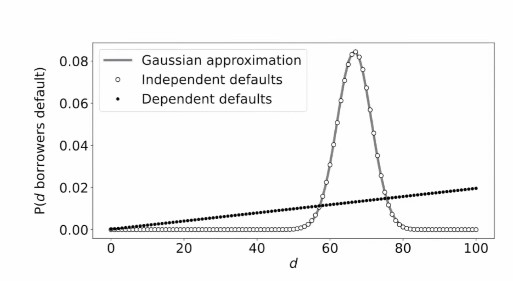
\includegraphics[width=10cm]{notes/week_4/vidio 3:How Not To Estimate Ris/immages/v_3_3.jpg}
\item so here we can see the likelihood that 90 percent of the defaults fail is non-negligible and this is because when the economy is bad everything fails 
\item so $P(d\geq .9n)=.187$ for n=100
\item and as n approach infinity $P(d\geq .9n)=.19$ so this thing stabilizes not at zero
\item so 20 percent of the time we get economic catastrophe in this model. 
\end{itemize}
\end{document}
